\documentclass[12pt,letterpaper]{article}
\usepackage{graphicx,textcomp}
\usepackage{natbib}
\usepackage{setspace}
\usepackage{fullpage}
\usepackage{color}
\usepackage[reqno]{amsmath}
\usepackage{amsthm}
\usepackage{fancyvrb}
\usepackage{amssymb,enumerate}
\usepackage[all]{xy}
\usepackage{endnotes}
\usepackage{lscape}
\newtheorem{com}{Comment}
\usepackage{float}
\usepackage{hyperref}
\newtheorem{lem} {Lemma}
\newtheorem{prop}{Proposition}
\newtheorem{thm}{Theorem}
\newtheorem{defn}{Definition}
\newtheorem{cor}{Corollary}
\newtheorem{obs}{Observation}
\usepackage[compact]{titlesec}
\usepackage{dcolumn}
\usepackage{tikz}
\usetikzlibrary{arrows}
\usepackage{multirow}
\usepackage{xcolor}
\newcolumntype{.}{D{.}{.}{-1}}
\newcolumntype{d}[1]{D{.}{.}{#1}}
\definecolor{light-gray}{gray}{0.65}
\usepackage{url}
\usepackage{listings}
\usepackage{color}

\definecolor{codegreen}{rgb}{0,0.6,0}
\definecolor{codegray}{rgb}{0.5,0.5,0.5}
\definecolor{codepurple}{rgb}{0.58,0,0.82}
\definecolor{backcolour}{rgb}{0.95,0.95,0.92}

\lstdefinestyle{mystyle}{
	backgroundcolor=\color{backcolour},   
	commentstyle=\color{codegreen},
	keywordstyle=\color{magenta},
	numberstyle=\tiny\color{codegray},
	stringstyle=\color{codepurple},
	basicstyle=\footnotesize,
	breakatwhitespace=false,         
	breaklines=true,                 
	captionpos=b,                    
	keepspaces=true,                 
	numbers=left,                    
	numbersep=5pt,                  
	showspaces=false,                
	showstringspaces=false,
	showtabs=false,                  
	tabsize=2
}
\lstset{style=mystyle}
\newcommand{\Sref}[1]{Section~\ref{#1}}
\newtheorem{hyp}{Hypothesis}

\title{Problem Set 3 Clare Zureich}
\date{Due: November 11, 2024}
\author{Applied Stats/Quant Methods 1}



\begin{document}
	\maketitle
	\section*{Instructions}
	\begin{itemize}
		\item Please show your work! You may lose points by simply writing in the answer. If the problem requires you to execute commands in \texttt{R}, please include the code you used to get your answers. Please also include the \texttt{.R} file that contains your code. If you are not sure if work needs to be shown for a particular problem, please ask.
	\item Your homework should be submitted electronically on GitHub.
	\item This problem set is due before 23:59 on Sunday November 11, 2024. No late assignments will be accepted.

	\end{itemize}

		\vspace{.25cm}
	
\noindent In this problem set, you will run several regressions and create an add variable plot (see the lecture slides) in \texttt{R} using the \texttt{incumbents\_subset.csv} dataset. Include all of your code.

	\vspace{.5cm}
\section*{Question 1}
\vspace{.25cm}
\noindent We are interested in knowing how the difference in campaign spending between incumbent and challenger affects the incumbent's vote share. 
	\begin{enumerate}
		\item Run a regression where the outcome variable is \texttt{voteshare} and the explanatory variable is \texttt{difflog}.	\vspace{1cm}
		
		There is a positive relationship between the amount of incumbent and challenger spending and the incumbent's vote share. The incumbent's vote share will, on average, increase by .04 for a one unit increase in the difference in spending (logged). The relationship is significantly significant as the p-value is low. 
		
		Below is the R Code and summary output of the regression: 
		\lstinputlisting[language=R, firstline=41, lastline=42]{PS03_answers_CZ.R}
		\includegraphics[width=.75\textwidth]{regression_summary1}
		
		\item Make a scatterplot of the two variables and add the regression line. 	
		
		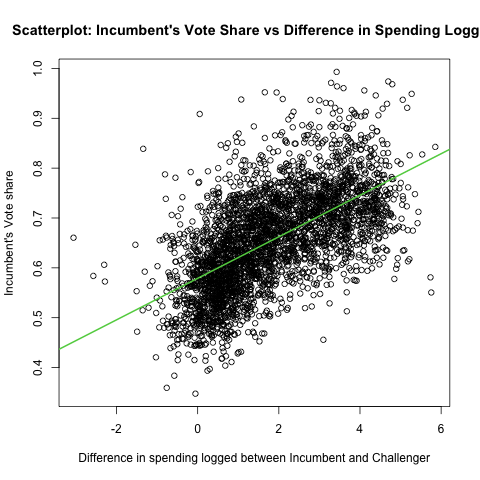
\includegraphics[width=.75\textwidth]{votesshare_vs_difflog.png}
		
		\lstinputlisting[language=R, firstline=46, lastline=51]{PS03_answers_CZ.R}
		
		
		\item Save the residuals of the model in a separate object.	\vspace{.1cm}
			\lstinputlisting[language=R, firstline=54, lastline=55]{PS03_answers_CZ.R}
				\includegraphics[width=.75\textwidth]{residual_summary1}
		\item Write the prediction equation. 
		$$\hat{y}= \hat{\beta_0} + \hat{\beta_1} \times \text{difflog}$$
		voteshare = 0.579 + 0.042 x difflog
		

		
	\end{enumerate}
	
\newpage

\section*{Question 2}
\noindent We are interested in knowing how the difference between incumbent and challenger's spending and the vote share of the presidential candidate of the incumbent's party are related.	\vspace{.25cm}
	\begin{enumerate}
		\item Run a regression where the outcome variable is \texttt{presvote} and the explanatory variable is \texttt{difflog}.	\vspace{.25cm}
		
		There is a positive relationship between the amount of incumbent and challenger spending and the presidential vote share. The presidential vote share will, on average, increase by .024 for a one unit increase in the difference in spending (logged). The relationship is significantly significant as the p-value is low. 
		
		Below is the R Code and summary output of the regression: 
		\lstinputlisting[language=R, firstline=63, lastline=64]{PS03_answers_CZ.R}
		\includegraphics[width=.75\textwidth]{regression_summary2}
		
		
		\item Make a scatterplot of the two variables and add the regression line. 	\vspace{.25cm}
		
			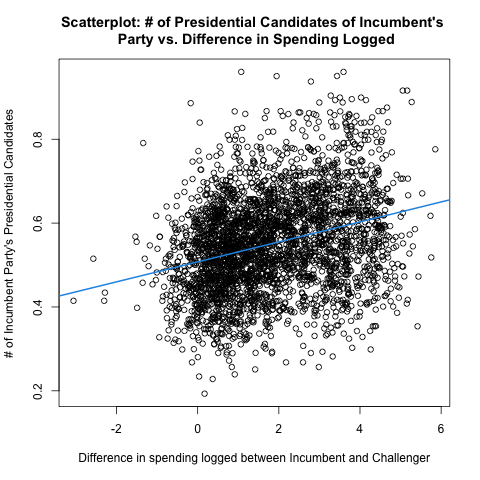
\includegraphics[width=.75\textwidth]{presvote_vs_difflog.png}
		\lstinputlisting[language=R, firstline=68, lastline=73]{PS03_answers_CZ.R}
		
		\item Save the residuals of the model in a separate object.	\vspace{.25cm}
		
	
		\lstinputlisting[language=R, firstline=76, lastline=77]{PS03_answers_CZ.R}
		\includegraphics[width=.75\textwidth]{residual_summary2}
		
		\item Write the prediction equation.
		$$\hat{y}= \hat{\beta_0} + \hat{\beta_1} \times \text{difflog}$$
		presvote = 0.508 + 0.024 x difflog
	\end{enumerate}
	
	\newpage	
\section*{Question 3}

\noindent We are interested in knowing how the vote share of the presidential candidate of the incumbent's party is associated with the incumbent's electoral success.
	\vspace{.25cm}
	\begin{enumerate}
		\item Run a regression where the outcome variable is \texttt{voteshare} and the explanatory variable is \texttt{presvote}.
			\vspace{.25cm}
			
			There is a positive relationship between the presidential vote share and the incumbent's vote share. The incumbent's vote share will, on average, increase by .388 for a one unit increase in the presidential vote share. The relationship is significantly significant as the p-value is low. 
			
			Below is the R Code and summary output of the regression: 
			\lstinputlisting[language=R, firstline=86, lastline=87]{PS03_answers_CZ.R}
			\includegraphics[width=.75\textwidth]{regression_summary3}
			
		\item Make a scatterplot of the two variables and add the regression line. 
			\vspace{.25cm}
			
			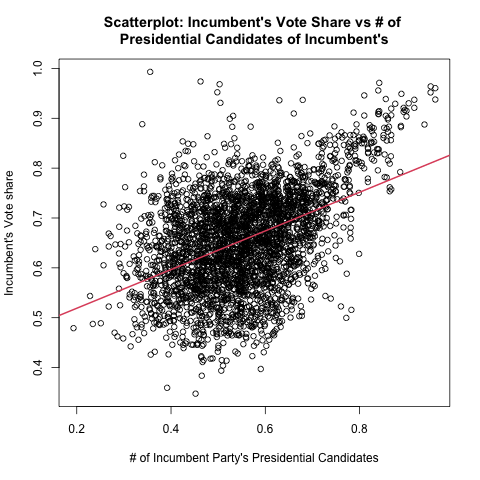
\includegraphics[width=.75\textwidth]{votesshare_vs_presvote.png}
			\lstinputlisting[language=R, firstline=91, lastline=96]{PS03_answers_CZ.R}
			
		\item Write the prediction equation.
		
		$$\hat{y}= \hat{\beta_0} + \hat{\beta_1} \times \text{presvote}$$
		voteshare = 0.441 + 0.388 x presvote
	\end{enumerate}
	

\newpage	
\section*{Question 4}
\noindent The residuals from part (a) tell us how much of the variation in \texttt{voteshare} is $not$ explained by the difference in spending between incumbent and challenger. The residuals in part (b) tell us how much of the variation in \texttt{presvote} is $not$ explained by the difference in spending between incumbent and challenger in the district.
	\begin{enumerate}
		\item Run a regression where the outcome variable is the residuals from Question 1 and the explanatory variable is the residuals from Question 2.	\vspace{.25cm}
		
		There is a positive relationship between the residuals from regression 1 (vote share vs difflog) and the residuals from regression 2 (presvote vs difflog). The residual error of regression 1 will, on average, increase by .257 for a one unit increase in regression 2 residuals error. The relationship is significantly significant as the p-value is low. 
		
		
		\lstinputlisting[language=R, firstline=105, lastline=106]{PS03_answers_CZ.R}
		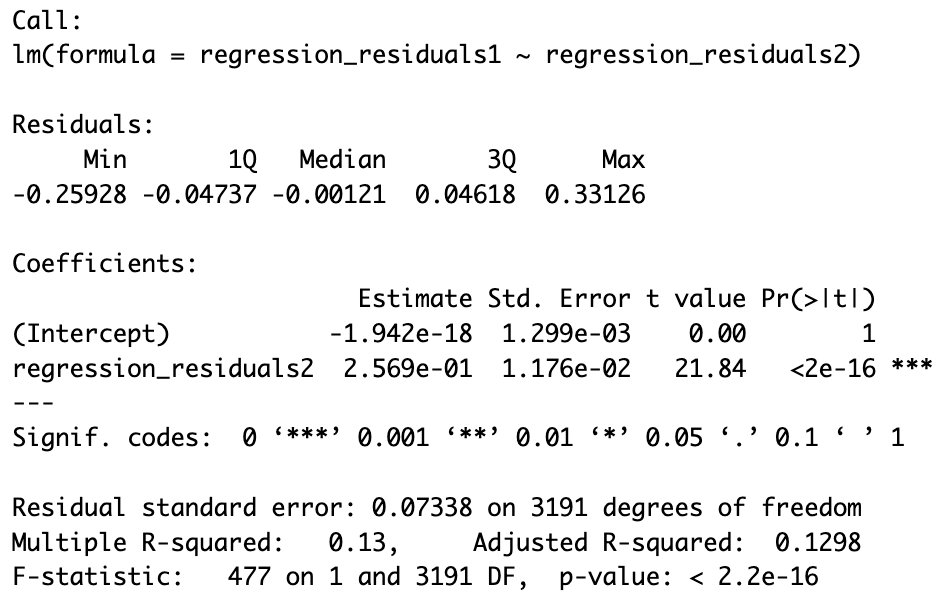
\includegraphics[width=.75\textwidth]{Residual_regression}

		
		\item Make a scatterplot of the two residuals and add the regression line. 	\vspace{6cm}
		
			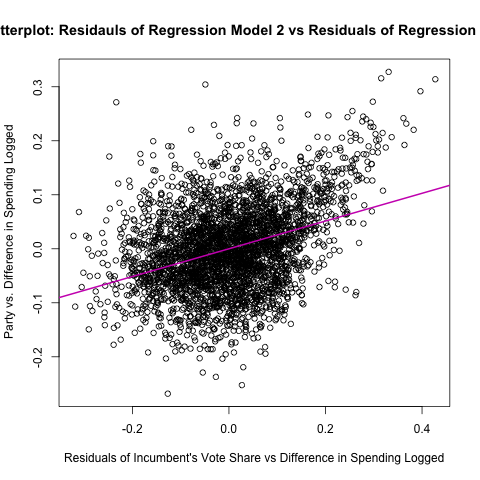
\includegraphics[width=.75\textwidth]{Q1_vs_Q2.png}
		\lstinputlisting[language=R, firstline=110, lastline=115]{PS03_answers_CZ.R}
		
		\item Write the prediction equation.
			$$\hat{y}= \hat{\beta_0} + \hat{\beta_1} \times \text{ResidualsQ2}$$
		ResidualsQ1= 0 + 0.257 ResidualsQ2
		
	\end{enumerate}
	
	\newpage	

\section*{Question 5}
\noindent What if the incumbent's vote share is affected by both the president's popularity and the difference in spending between incumbent and challenger? 
	\begin{enumerate}
		\item Run a regression where the outcome variable is the incumbent's \texttt{voteshare} and the explanatory variables are \texttt{difflog} and \texttt{presvote}.	\vspace{.25cm}
		
		
		\lstinputlisting[language=R, firstline=123, lastline=124]{PS03_answers_CZ.R}
		\includegraphics[width=.75\textwidth]{regression_summary5}
		
		\item Write the prediction equation.	\vspace{.25cm}
		
			$$\hat{y}= \hat{\beta_0} + \hat{\beta_1} \times \text{difflog}+ \hat{\beta_2} \times \text{presvote}$$
		voteshare = .449 + .036 x difflog + .257 x presvote
		
	
		\item What is it in this output that is identical to the output in Question 4? Why do you think this is the case?
		
	The slope coefficient of the regressionresidual2 variable in the residual regression model (.257) is equal to the slope coefficient of the presvote variable in the multivariate linear model (and prediction equation) (.257). This is because the slope coefficients in both models represent the effect of presvote on voteshare after taking out the effects of difflog from both voteshare and presvote. This is the partial effect of presvote. 
		
	Step by step analysis: 
	In regressionresiduals1, we first found the residual of the linear relationship between votesahre and difflog (regressionmodel1), which is the part of voteshare that is not linearly related to difflog. In regressionresiduals2, we found the residual of the linear relationship between presvote and difflog (regressionmodel2), which is the part of presvote that is not linearly related to difflog.  We then found the linear relationship between the voteshare residual (regressionresidual1) and the presvote residual (regressionresidual2). The result is the coefficient which represents the effect of presvote on voteshare after taking out the effects of difflog from voteshare and presvote.
		
	\end{enumerate}




\end{document}
